\section{Generación del Código de los Componentes y Procedimientos}
 \noindent Este documento describe el diseño de la lógica de programación y los algoritmos utilizados para la solución de los diversos problemas que implicaba la generación del código de los componentes de SisPAF.\\
 
 \noindent SisPAF es un sistema compuesto por 3 módulos principales, cada uno contando con su propio desarrollo para la interfaz y para el código que acompaña dicha interfaz. La figura X ilustra el modelo lógico del sistema donde se pueden observar los 3 módulos antes mencionados, los cuales son:\\
 
 \subsubsection{Búsqueda de información:}\label{Busqueda}
 \noindent El módulo de búsqueda de información es el primer módulo de SisPAF y es el encargado de obtener la información necesaria para realizar la predicción de la actividad farmacológica (efectividad de los fármacos frente a cierta patología).\\
 
 \subsubsection{Análisis de la información:}
\noindent Una vez obtenidos los datos del módulo de búsqueda y que el usuario es informado de los resultados de dicha búsqueda, se procede a realizar un análisis de la información obtenida. Para esto se empleo el uso de un método de la bioinformática conocido como modelo QSAR (por sus siglas en inglés, \textit{Quantitative Structure Activity Relationship}) que permite relacionar a los compuestos con determinadas proteínas y predecir qué tan efectivos pueden ser para atacar y destruir esas proteínas. Dentro del mismo modelo QSAR se utilizan algoritmos de \textit{Machine Learning}, en este caso regresión lineal múltiple y mapa auto-organizado para generar los resultados que representan la efectividad de los compuestos, previamente mencionada.

\subsubsection{Generación de resultados:}
\noindent En este módulo, los resultados del análisis son ordenados y desplegados al usuario en una interfaz, para su visualización con opción a ser almacenados en el sistema.

\begin{figure}[H]
    \centering
    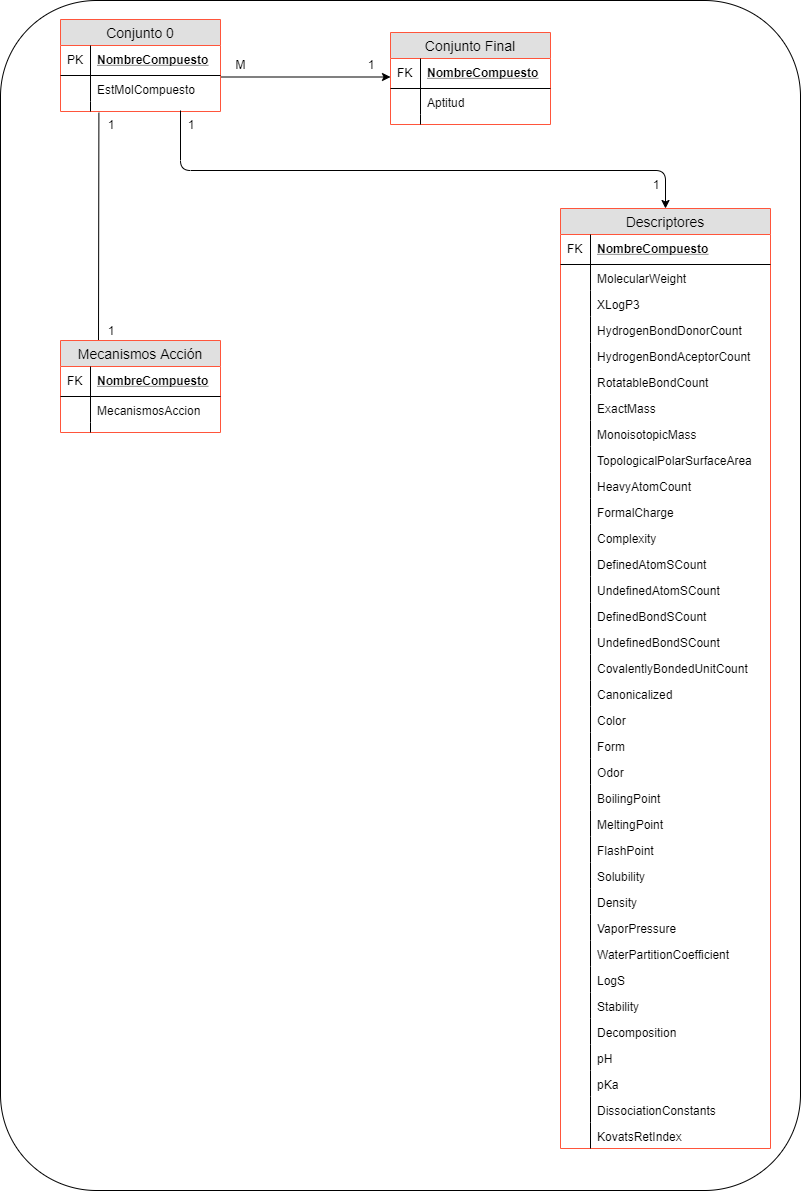
\includegraphics[scale=0.40]{Capitulo4/Documentos/imagenes_generacion/modeloDatosLogico.png}
    \caption{Modelo lógico de SisPAF.}
    \label{Modelo_logico_de_SisPAF_1}
\end{figure}

\subsubsection{Generación de código de los componentes}
\subsection{Búsqueda de información}
\noindent Este módulo incluye desde la ventana de inicio de SisPAF (descrita en el apartado \ref{Busqueda}) hasta la confirmación de los resultados de la búsqueda. El usuario ingresa un archivo inicial (véase en la tabla \ref{diccionario}) o indica un directorio donde se encuentre un proyecto ya existente.  SisPAF analiza ya sea el directorio o el archivo inicial y recopila información sobre los compuestos y proteínas de los que se desean obtener datos en específico (estructura molecular de los compuestos, estructura molecular de las proteínas, descriptores físico químicos de los compuestos, mecanismos de acción de los compuestos). Cuando SisPAF determina los elementos (compuestos y proteínas indicados por el usuario) de los cuales debe obtener dichos datos, realiza las conexiones correspondientes con las bases de datos en línea que proveen esa información (en la figura \ref{DFD1} se observan las 3 bases de datos, DrugBank, PDB,  PubChem, y la información que de ellas se obtiene). Finalmente se despliega al usuario una tabla con un resumen de qué datos se obtuvieron para cada uno de los elementos identificados.\\

\noindent El diagrama de flujo que ilustra la figura \ref{DFD1}. muestra las actividades que componen al módulo de búsqueda de información, las cuales de describen a continuación.

\begin{figure}[H]
    \centering
    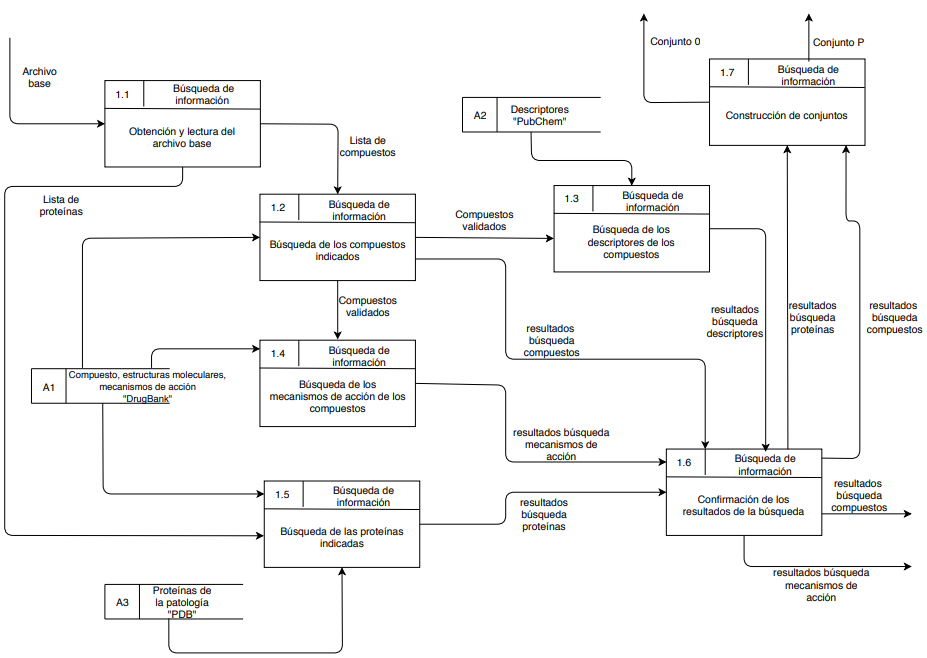
\includegraphics[scale=0.46]{Capitulo2/images/DFD-1.png}
    \caption{Diagrama de flujo de datos del módulo de búsqueda de información.}
    \label{DFD1}
\end{figure}
%%%%%%%%%%%%%%%%%%%%%%%%%%%%%%%%%%%%%%%%%%%%%%%%%%%%%%%%%%%%%%%
\subsubsection{Diseño de interfaces}{
\noindent Al momento de  realizar el análisis y diseño del sistema de información,  se plantearon las vistas que tendrían las interfaces, empezando por las que comunican al usuario con las funciones más importantes del sistema, como la adquisición del archivo inicial, si existe un  error en este, entre otras interacciones importantes al iniciar SisPAF.\\

\noindent A continuación mostramos las pantallas que se consideran importantes, y el resultado al ser programadas en el lenguaje Python, auxiliándose en la librería Tkinter.

\begin{figure}[H]
    \centering
    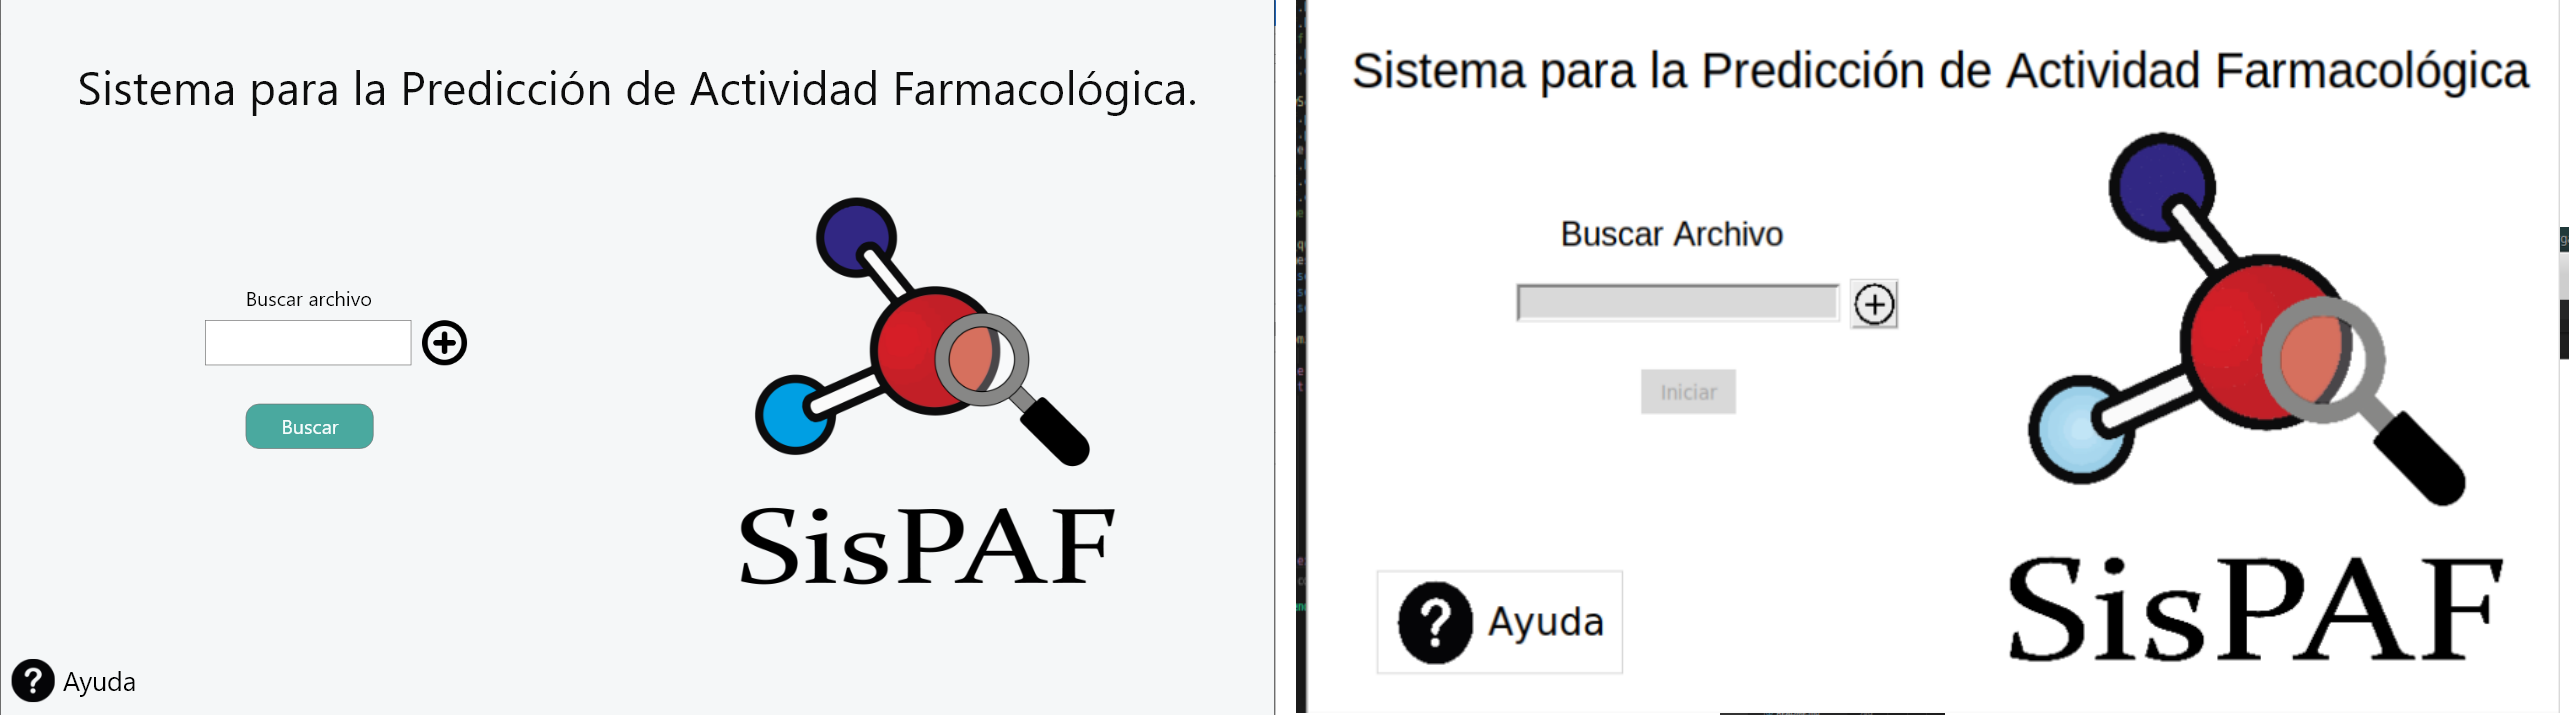
\includegraphics[scale=0.215]{Capitulo4/Documentos/imagenes_generacion/ComparacionPan1.png}
    \caption{Comparación de pantallas, a la izquierda la diseñada y  a la derecha la pantalla programada.}
    \label{comparacion}
\end{figure}

\noindent A esas pantallas se han incluido mensajes de error, que igual estaban planificados para cuando existieran posibles fallos, uno de ellos, es cuando el archivo no contiene el formato y/o contenido adecuado.\\

\begin{figure}[H]
    \centering
    
\includegraphics[scale=0.375]{Capitulo4/Documentos/imagenes_generacion/PickwrongAr.png}
    \caption{Comparación de mensajes de error, a la izquierda la planeada y a la derecha la programada.}
    \label{comparacion_2}
\end{figure}

}
%%%%%%%%%%%%%%%%%%%%%%%%%%%%%%%%%%%%%%%%%%%%%%%%%%%%%%%%%%%%%%
\subsubsection{Inicio}{
\noindent La interfaz de inicio funciona como una especie de canalizador. Dependiendo de si el usuario quiere crear un nuevo proyecto o abrir uno ya existente, los procesos a ejecutar son diferentes hasta que se llega a la parte del análisis de información. Para comenzar, cualquier botón solicita al usuario que seleccione un directorio (para crear o para abrir un proyecto). Si se desea crear un nuevo proyecto se procede a mostrar la interfaz correspondiente que le permite al usuario cargar al sistema un archivo inicial y comenzar con el proceso de la búsqueda de información. Por otro lado si el usuario elige abrir un proyecto el sistema solicita que se le indique el directorio donde se encuentra dicho proyecto y procede a analizar la estructura del directorio para definir la información que ya se ha obtenido y continuar el proceso desde el punto necesario.\\
}
%%%%%%%%%%%%%%%%%%%%%%%%%%%%%%%%%%%%%%%%%%%
\subsubsection{Obtención y lectura del archivo inicial}{
\noindent El proceso para realizar la obtención y la lectura del archivo inicial (véase \ref{diccionario}) involucra la comunicación de la interfaz que es la que determina dónde se va a almacenar dicho archivo y el uso de herramientas básicas de lectura y escritura presentes en python. Python permite abrir un archivo simplemente con especificar la ruta donde se encuentra almacenado. Luego se realiza la lectura del archivo mediante un ciclo que lee línea por línea hasta que se encuentra con el final de dicho archivo. Durante esta lectura es donde es posible almacenar la información requerida en dos secciones separadas, en este caso una sección para compuestos y una para proteínas. Estos dos apartados definen los elementos cuya información debe ser buscada en la base de datos en línea.
En este proceso se hace presente la comprobación de la estructura del archivo inicial, la cual es representada de manera gráfica por la figura \ref{flujo}.\\


\noindent La figura \ref{flujo} contiene el diagrama de flujo para el proceso de comprobación del archivo inicial, el cual se basa en revisar la presencia de las etiquetas (Compounds y Proteins) y enviar una alerta al usuario en caso de que no se encuentren dichas etiquetas. El mismo SisPAF, al momento de leer y almacenar la información del archivo inicial, es capaz de detectar elementos duplicados, haciendo que los elementos obtenidos sean únicos.

\begin{figure}[H]
    \centering
    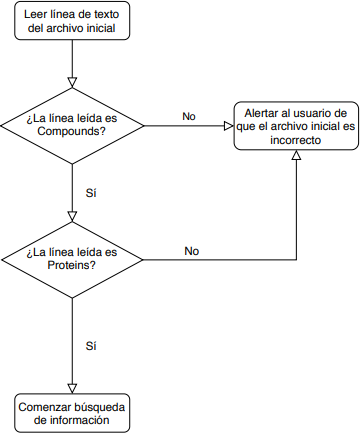
\includegraphics[scale=0.85]{Capitulo4/imagenes/diagramaArchivoInicia.png}
    \caption{Diagrama de flujo del análisis del archivo inicial.}
    \label{flujo}
\end{figure}
}
%%%%%%%%%%%%%%%%%%%%%%%%%%%%%%%%%%%%%%%%%%%%%%%%%%%%%
\subsubsection{Diseño de interfaces}{
\noindent Para el módulo de la búsqueda de datos, se diseñaron interfaces que muestran el status del sistema durante la conexión a las bases de datos, mostrar el resultado de dichas consultas, dándole a saber al usuario si hubo un error en la adquisición de la información necesario de los compuestos o las proteínas.\\

\noindent A continuación se muestra la pantalla de espera, mientras el sistema realiza la búsqueda de información, con la cual se le indica al usuario que el sistema sigue trabajando.
}

\begin{figure}[H]
    \centering
    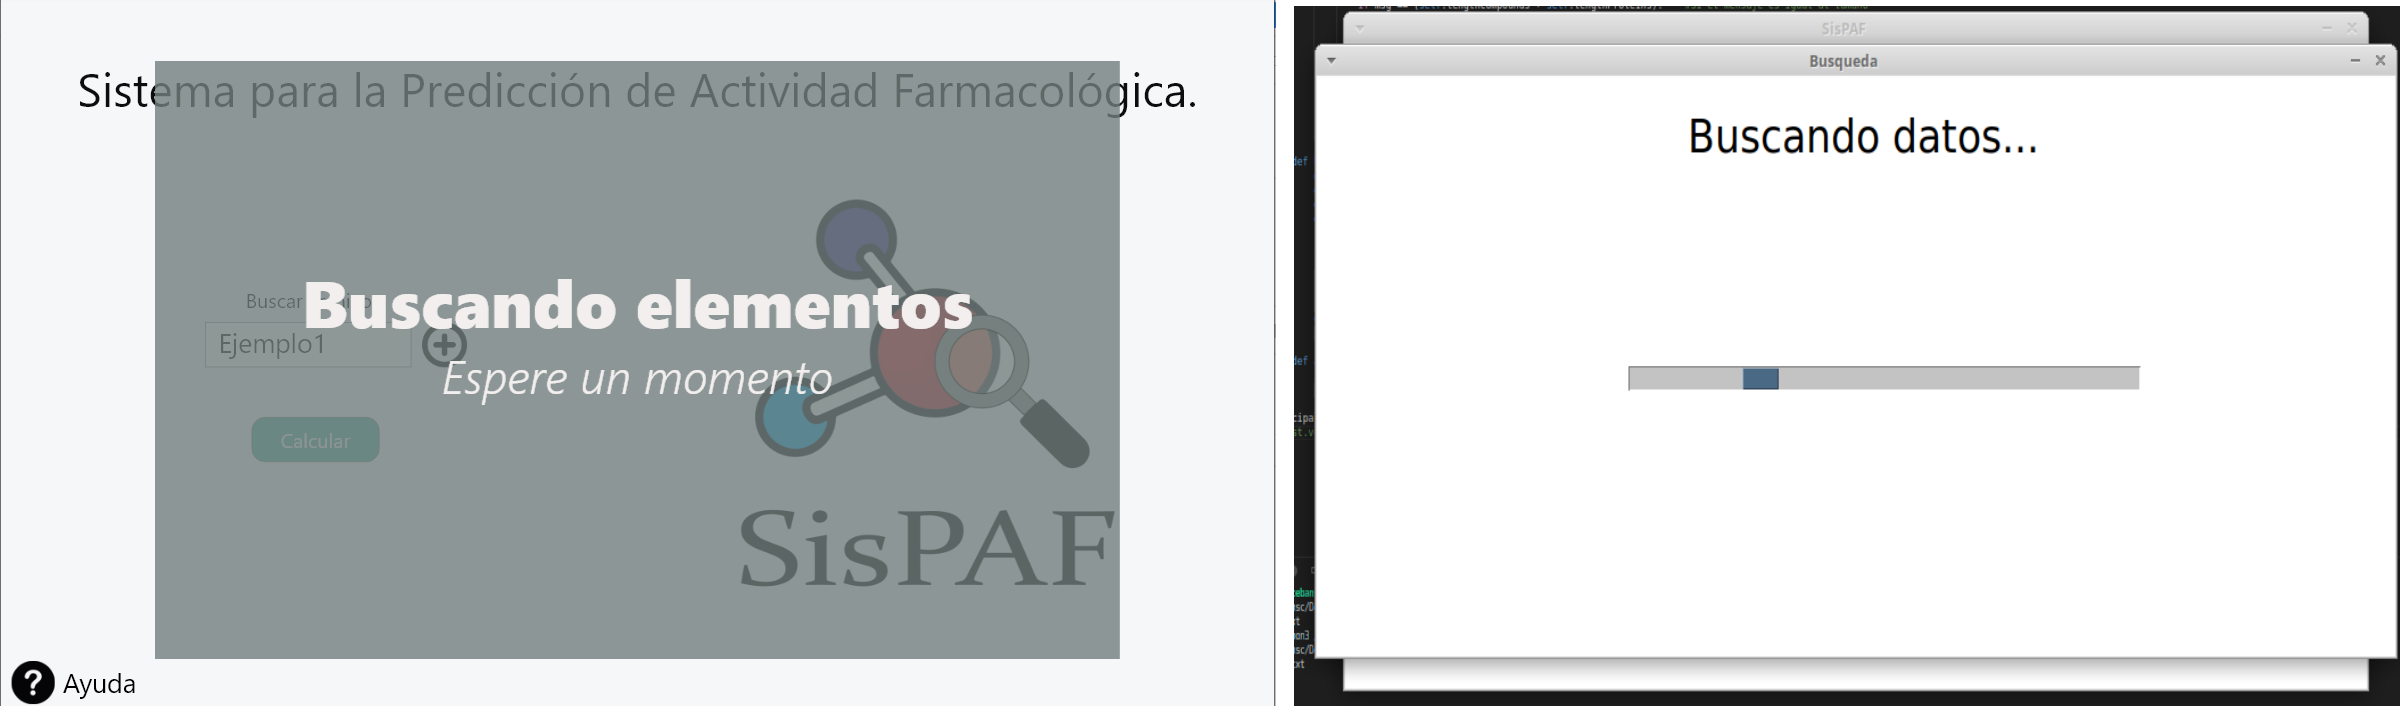
\includegraphics[scale=0.235]{Capitulo4/Documentos/imagenes_generacion/Esperabusqueda.png}
    \caption{Comparación de pantallas de espera para la búsqueda de información, a la izquierda la planeada y a la derecha la programada.}
    \label{comparacion_3}
\end{figure}

\noindent Durante la búsqueda, el mayor problema, incluso considerarse fatal, sería la pérdida de conexión a internet, para ello se planeó en un inicio la aparición de un mensaje de error para cuando esto suceda.

\begin{figure}[H]
    \centering
    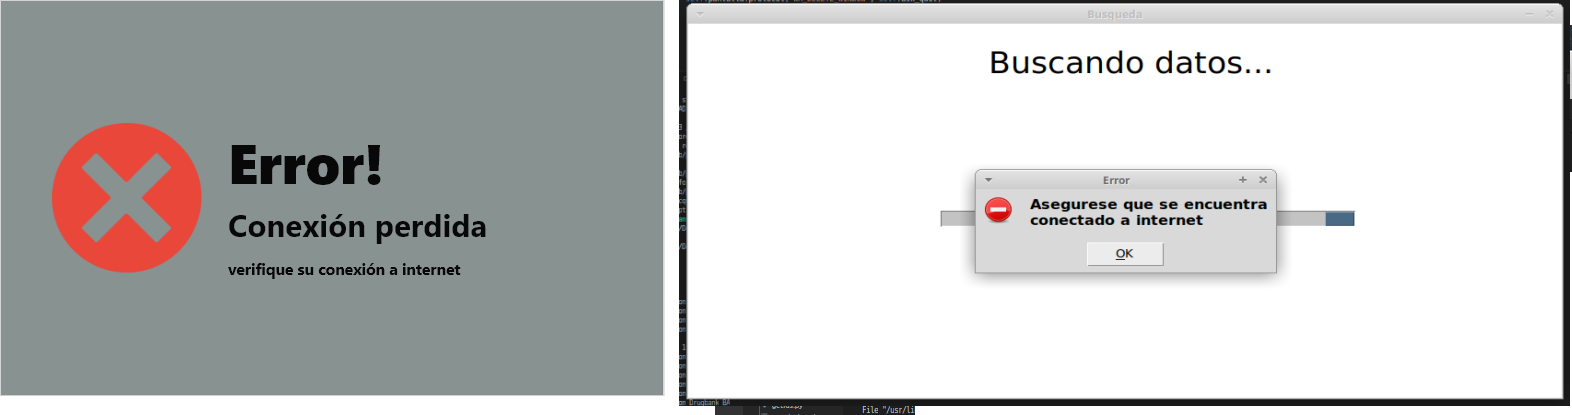
\includegraphics[scale=0.375]{Capitulo4/Documentos/imagenes_generacion/errorNet.png}
    \caption{Comparación de mensajes de error en la pérdida de conexión, a la izquierda la planeada y a la derecha la programada.}
    \label{comparacion_4}
\end{figure}

\noindent Cuando la búsqueda de datos, ha finalizado, al usuarios se muestra una pantalla que indica el estado de cada compuesto y proteína respecto a la información que nos interesa de ellos, si no se encontró la estructura del compuesto, o de la proteína, etc.

\begin{figure}[H]
    \centering
    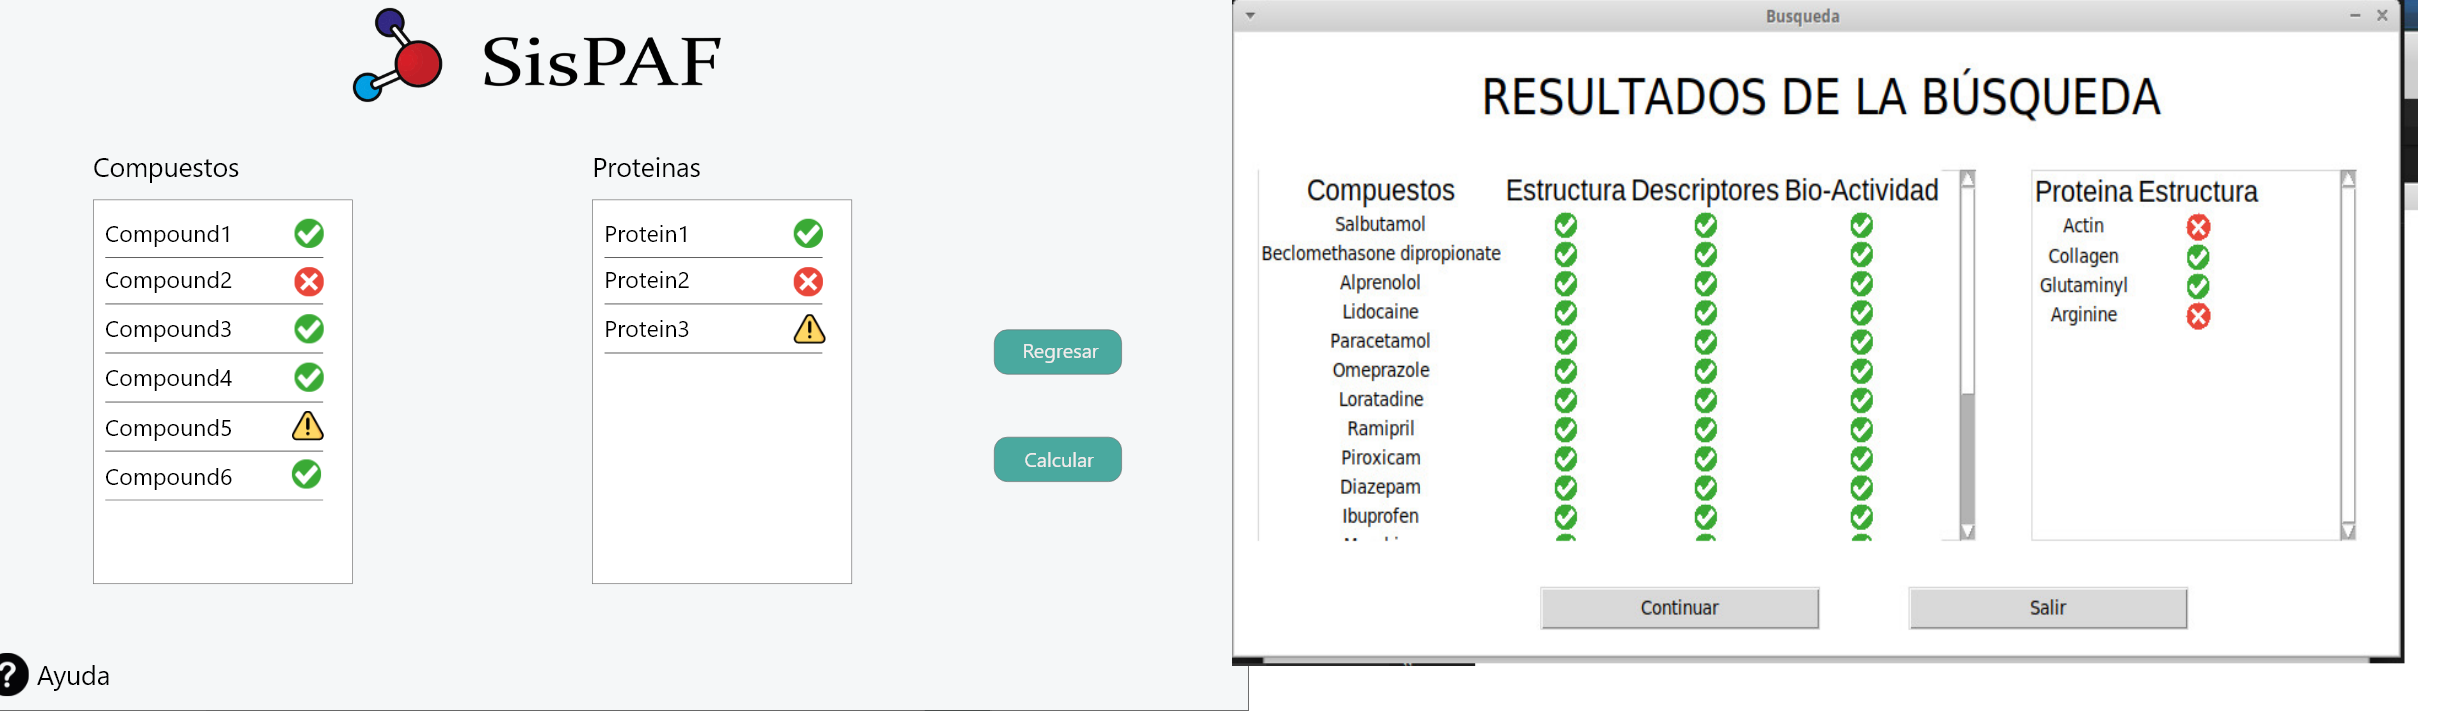
\includegraphics[scale=0.225]{Capitulo4/Documentos/imagenes_generacion/ResultBusqueda.png}
    \caption{Comparación de pantallas para resultados de búsqueda, a la izquierda la planeada y a la derecha la programada.}
    \label{comparacion_5}
\end{figure}
%%%%%%%%%%%%%%%%%%%%%%%%%%%%%%%%%%%%%%%%%%%%%%%%%%%%%%%%%%%%%%
\subsubsection{Búsqueda de información: uso de API’s y Web scrapping}
\noindent Cuando ya se han definido los elementos de los cuales se debe obtener su información, se procede a utilizar API’s que las bases de datos en línea poseen y que utilizan para consultar la información de dichas bases de datos. Para realizar las llamadas a las API se deben tomar en cuenta dos cosas: la cantidad límite de peticiones por segundo que cada API define para evitar saturarse de solicitudes y la manera en cómo debe accederse a la información que se requiere obtener (para este caso, la estructura molecular, los descriptores fisicoquímicos computados y los mecanismos de acción para cada uno de los  compuestos, mientras que para las proteínas solo se requiere la estructura molecular).

\noindent En esta situación python provee de bibliotecas que permiten realizar las peticiones a las API de una forma más sencilla y eficaz que de la manera tradicional, pues dichas bibliotecas están enfocadas solo a trabajar con las API’s de las bases de datos en cuestión (PDB, PubChem).

\noindent Para el caso de las proteínas, el dato de mayor importancia, es su estructura, la cual se requiere en formato pdb, que brinda la suficiente información de la proteína para realizar todos cálculos necesarios,  al requerirse un formato pdb, nos valemos de la base de datos de Protein Data Bank, el proceso de obtención, consiste en adquirir el nombre de la proteína, comparar de entre todas las proteínas existentes en la base de datos el nombre exacto de la proteína que empate mejor con la proporcionada por el usuario, cuando ya se obtiene un nombre, se consigue el ID de PDB para poder obtener todo el archivo que contiene la estructura, es un poco mejor visualizado en el diagrama.\\


\begin{figure}[H]
    \centering
    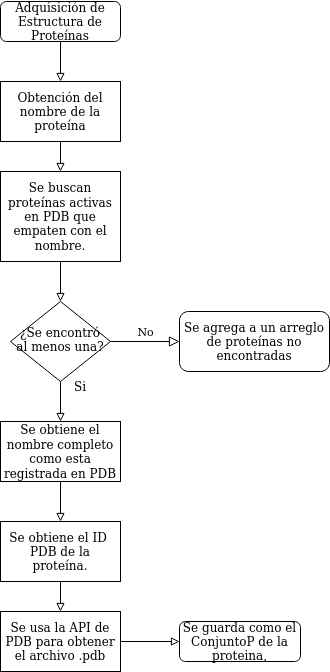
\includegraphics[scale=0.75]{Capitulo4/Documentos/imagenes_generacion/EstructuraPro.png}
    \caption{Diagrama de flujo de adquisición de la estructura de  Proteínas}
    \label{Adquisicion_estructura}
\end{figure}

\noindent Para el caso de la base de datos DrugBank, si bien es de libre acceso, su API no lo es, por lo que, para obtener información de los elementos contenidos en dicha base de datos se utiliza un método conocido como Web Scraping. 

\noindent Para realizar el método ya mencionado es usada la librería Selenium, este técnica es únicamente usada para adquirir la estructura pdb del compuesto, así como su actividad biológica.  Algo más que se debe aclarar es que para trabajar con Selenium es usado un driver para ser ocupado sobre un navegador web.\\

\noindent Para la adquisición de la estructura PDB, se ingresa a la página de drugbank, se realiza la búsqueda del compuesto, si éste existe, se procede a obtener un elemento html que  nos brinde la  dirección  web, a la cual se realiza un  request para conseguir su contenido, que es la estructura del compuesto. Esto queda mejor explicado en el siguiente diagrama.\\

\begin{figure}[H]
    \centering
    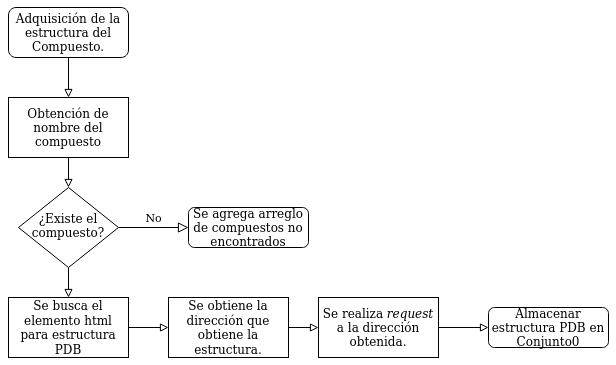
\includegraphics[scale=0.70]{Capitulo4/Documentos/imagenes_entorno/figura_flujo.png}
    \caption{Diagrama de flujo de adquisición PDB del compuesto haciendo uso de Web Scrapping.}
    \label{Diagrama_de_flujo_1}
\end{figure}

\noindent Junto con la estructura, la bio-actividad se adquiere por medio de  Drugbank y haciendo uso del Web Scrapping, una vez que se cuenta con el nombre del compuesto, se busca la sección de Actividad Biológica, para esto  de igual forma, ya se debe haber confirmado en el mismo proceso si el compuesto  existe. si en la página que muestra toda la información del compuesto, no se halla la sección deseada, se indica en  el archivo del conjunto 0 que no posee actividad, de existir la sección, se obtiene el contenido de la tabla, se realiza la conversión a una cadena de caracteres para ser guardada en el archivo  conjunto 0.

\begin{figure}[H]
    \centering
    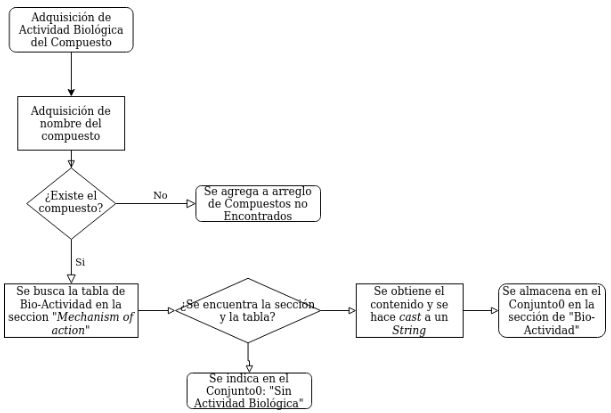
\includegraphics[scale=0.70]{Capitulo4/Documentos/imagenes_entorno/Actividad_biologica.png}
    \caption{Diagrama de flujo de adquisición de la Actividad Biológica}
    \label{Actividad_biologica}
\end{figure}

%%%%%%%%%%%%%%%%%%%%%%%%%%%%%%%%%%%%%%%%%%%%%%%%%%%%%%%%5
\subsubsection{Búsqueda concurrente}\label{concurrente}
\noindent El proceso de solicitar información a las API o realizar web scrapping, si bien no es complejo puede llegar a tomar algo de tiempo para recibir una respuesta del servidor que tienen las bases de datos. Para solucionar esta situación se utiliza la programación concurrente con hilos, los cuales evitan la latencia provocada por los tiempos que demoran las API en resolver las solicitudes que envía SisPAF. El programa crea un hilo por cada elemento que se obtuvo con la lectura del archivo inicial (tanto de compuestos como de proteínas). Cada hilo entonces tiene un elemento asociado del cual debe conseguir información mediante las peticiones a las API o el uso de web scrapping. Así, el tiempo requerido para realizar la búsqueda de información se reduce considerablemente.

\subsubsection{Construcción de conjuntos}
\noindent A la par de la actividad de búsqueda, una vez que la información es obtenida mediante las API’s, los hilos proceden a escribir esa información en archivos de texto. Para los compuestos, los hilos escriben la información en archivos de texto plano dentro de un directorio denominado Compounds, el cual está en el directorio donde se ha creado (o donde ya existe) el proyecto. Por su parte, la información de las proteínas es almacenada de la misma forma, solo que en un directorio de nombre Proteins. Los archivos que comprende el directorio Compounds forman el conjunto 0 (Véase \ref{diccionario}), mientras que todos los archivos que se encuentran en el directorio de Proteins forman el conjunto P (véase \ref{diccionario}).

\subsubsection{Manejo de pérdida de conexión a internet}
\noindent El manejo del error de conexión a internet está compuesto por tres partes. La primera parte es la detección de desconexión, que se realiza cuando alguna de las API’s o el proceso de webscrapping arrojan un error que se identifica como error de red. La segunda parte que toma lugar luego de que el error de red es identificado, es la de alerta al usuario de que no hay conexión a internet a la vez que se suspende el proceso de búsqueda, es decir, mientras no haya conexión las peticiones a las API’s y el webscrapping no son realizados pues los hilos se encuentran “dormidos”. La tercera parte es la reconexión la cual sucede cuando el usuario atiende la alerta emitida por el sistema, el cual como respuesta, realiza una rápida comprobación verificando si le es posible acceder al servidor central de Google. En caso de que le sea posible, el sistema emite una notificación para que todos los hilos que se encontraban pausados continúen con el proceso de la búsqueda de datos. Si por el contrario no es posible realizar la conexión al servidor de Google, la alerta vuelve a aparecer y el proceso de búsqueda se mantiene suspendido. La figura \ref{Desconexion} muestra el diagrama de flujo que sirvió como base para implementar la solución descrita en este apartado.

\begin{figure}[H]
    \centering
    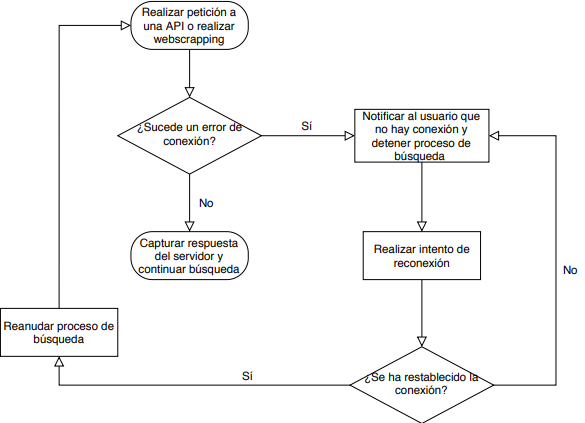
\includegraphics[scale=0.7]{Capitulo4/imagenes/diagramaDesconexion.png}
    \caption{Diagrama de flujo para el manejo de la pérdida de conexión a internet}
    \label{Desconexion}
\end{figure}

\subsubsection{Lectura de contenido de un proyecto}
\noindent Para el caso en el que el usuario desea abrir un proyecto ya existente, SisPAF solicita primero que se le indique el directorio donde se encuentra el proyecto. Acto seguido analiza la estructura de ese directorio para revisar que contenga los archivos que deben estar ahí puesto que si ya se ha creado un proyecto en ese directorio, deben existir ahí por lo menos el directorio de Compounds, el de Proteins y la copia del archivo inicial que genera el sistema (estos elementos se generan cuando se crea un nuevo proyecto). Si existen estos elementos procede a analizar el contenido de dichos directorios para determinar qué archivos faltan y que archivos se encuentran incompletos y requieren más información (esta lectura se realiza utilizando hilos para optimizar la tarea de leer varios archivos, se sigue la idea descrita en el apartado \ref{concurrente}). Una vez hecho esto se procede a continuar con el proceso ya sea de búsqueda o análisis dependiendo de la robustez actual del proyecto en cuestión. Si el sistema detecta un archivo final (Tabla \ref{diccionario}) no procede a abrir dicho proyecto pues este archivo es la muestra de que el proyecto ya ha sido terminado. La figura \ref{abrir} describe el diagrama de flujo que sigue el proceso de abrir un proyecto existente.

\begin{figure}[H]
    \centering
    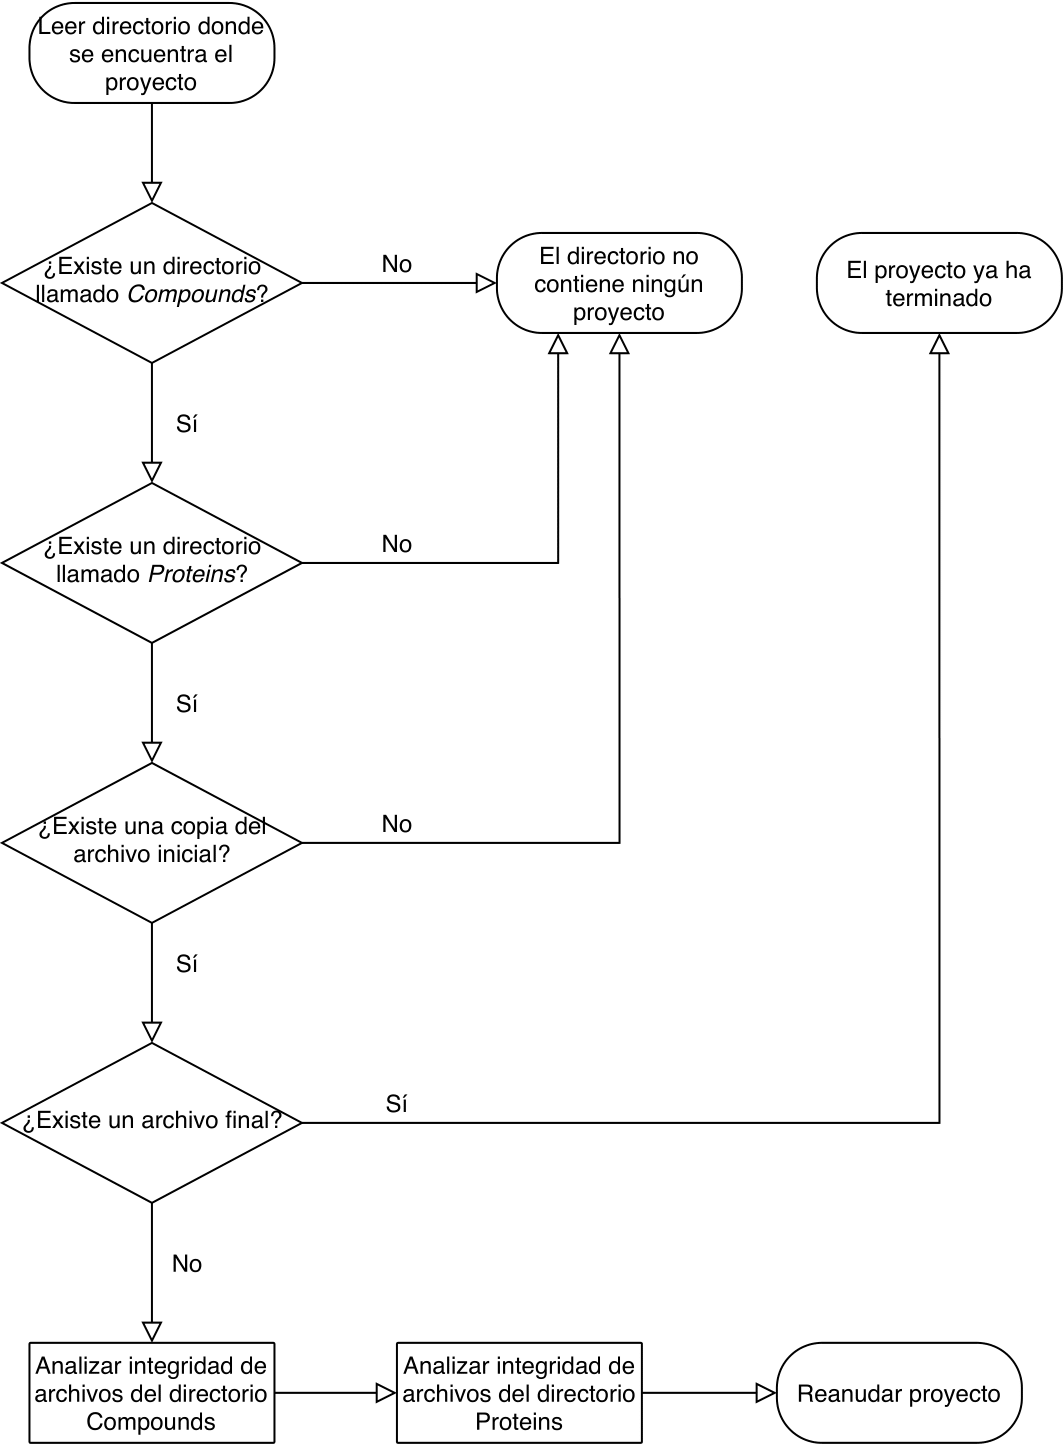
\includegraphics[scale=0.3]{Capitulo4/imagenes/diagramaAbrirProy-1.png}
    \caption{Diagrama de flujo que sigue SisPAF cuando se solicita abrir un proyecto ya existente.}
    \label{abrir}
\end{figure}
%%%%%%%%%%%%%%%%%%%%%%%%%%%%%%%%%%%%%%%%%%%%%%%%%%%%%
\subsection{Análisis de información}
\subsubsection{Diseño de interfaces}{
\noindent En la sección de análisis, donde el sistema hace uso de toda la información recolectada, se planificó una interfaz muy similar a la que se muestra durante el proceso de la búsqueda de información, una pantalla de espera,  para hacerle saber al usuario que el sistema  continúa trabajando, la comparación se muestra a continuación.

\begin{figure}[H]
    \centering
    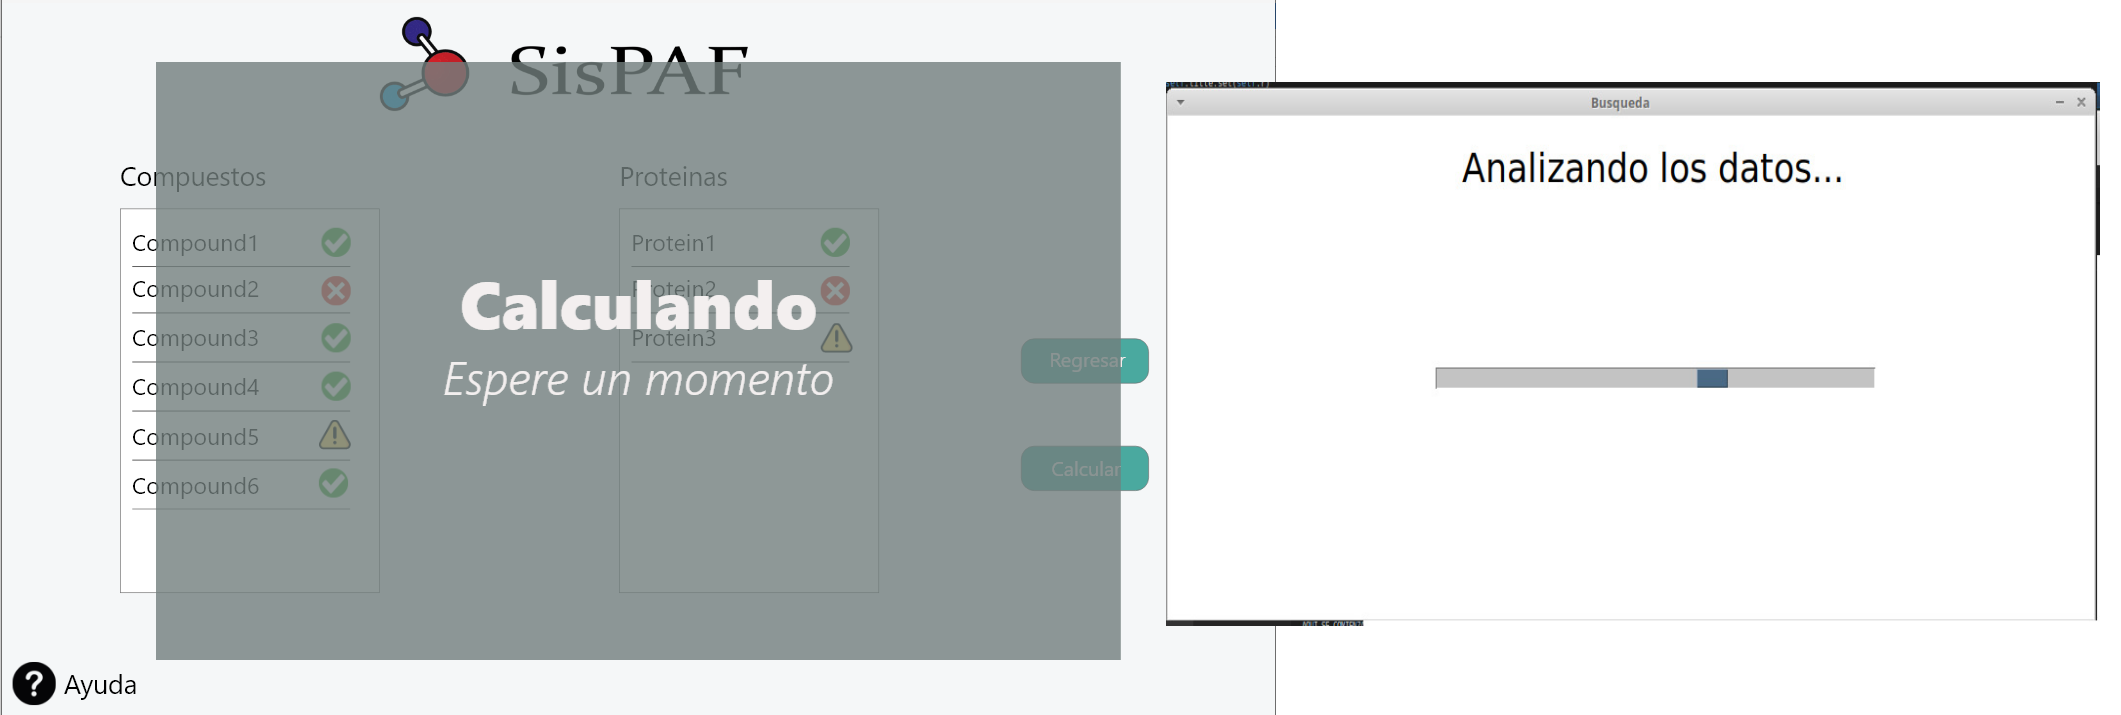
\includegraphics[scale=0.27]{Capitulo4/Documentos/imagenes_generacion/Analisis.png}
    \caption{Comparación de pantallas para el análisis de datos, a la izquierda la planeada y a la derecha la programada.}
    \label{comparacion_6l}
\end{figure}
}
\subsubsection{Análisis multiproceso}{
\noindent El desarrollo del proceso del análisis de la información es considerado exhaustivo de CPU, es decir, este proceso requiere una considerable capacidad de procesamiento del equipo de cómputo. Contrario a la aplicación concurrente con hilos, para los procesos que involucran en uso considerable de recursos de procesamiento se emplea el método de multiprocesos. El uso de múltiples procesos para el módulo de análisis de información supone una reducción considerable en los tiempos de procesamiento. Aquí se toman en cuenta dos cosas, la primera es la cantidad de procesos y la división de tareas, ya que el número de procesos que se debe crear corresponde con el número de núcleos físicos del equipo de cómputo, y a su vez las tareas a realizar deben asignarse a cada uno de los procesos creados. La segunda cosa a tomar en cuenta es la ventaja de un trabajo en paralelo. El uso de múltiples procesos permite una paralelización de las actividades que debe realizar el sistema, es decir, si se tienen 4 núcleos, se pueden realizar al mismo tiempo (de manera paralela) 4 actividades, aprovechando al 100\% la capacidad de procesamiento del equipo de cómputo donde se está ejecutando el sistema.



}
\subsubsection{\textit{Docking}}{
\noindent En el campo de modelado molecular (acoplamiento molecular) es un método que predice la conformación preferida de una molécula, al estar unida a otra, con el fin de formar un complejo estable.\cite{15}\\
\noindent La simulación de este procedimiento es un proceso complicado. En este enfoque, la proteína y el ligando están separados por una distancia física, y el ligando encuentra su posición en el sitio activo de la proteína luego de un cierto número de ''movimientos'' en su espacio conformacional. Los movimientos incorporan al cuerpo rígido transformaciones tales como el traslado y rotaciones. Cada uno de estos movimientos, en el espacio conformacional del ligando, induce un costo energético al sistema, y por tanto después de cada movimiento, se calcula la energía total del sistema.\\

\noindent Para hacer un examen de acoplamiento, primero se necesita la estructura de la proteína. Normalmente la estructura ha sido determinada usando una técnica biofísica como la cristalografía de rayos X, o menos frecuente, una Espectroscopia de resonancia magnética nuclear. La estructura de esta proteína y la de los ligandos potenciales sirven como los valores a ingresar en el programa que calcula el acoplamiento. El éxito del programa depende de dos factores: el algoritmo de búsqueda y la función de puntuación.\\

\noindent Para el acoplamiento molecular usamos una herramienta llamada AutoDock Vina la cual permite calcular de manera automática cada uno de estos movimientos. Para generar el resultado de \textit{Docking} con vina, pide como parámetros un archivo donde se configuran las entradas al sistemas y que esperas como salida del mismo, un ejemplo de este archivo, está ilustrado en la figura \ref{dock_ing}.\\

\noindent Como salida tendremos un archivo PDBQT el cual nos da el valor del acoplamiento molecular en distintas iteraciones, a estos valores los llamaremos “Deltas” los cuales son una pieza fundamental para implementar el algoritmo de regresión lineal, ya que estos datos se convertirán en nuestra variable dependiente.

\begin{figure}[H]
    \centering
    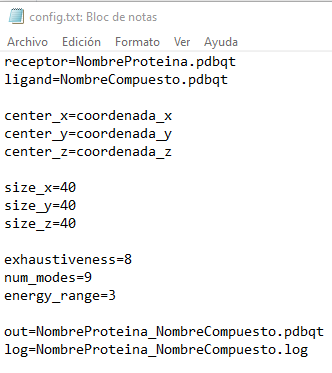
\includegraphics[scale=.99]{Capitulo4/Documentos/imagenes_entorno/archivo_entrada.png}
    \caption{Archivo de configuración para\textit{Docking}.}
    \label{dock_ing}
\end{figure}

\noindent Como podemos ver, Vina pide como parámetros de entrada la estructura 3D de un receptor (molécula que recibe, por lo normal es una proteína u otro biopolímero) y la estructura 3D del ligando (molécula que se enlaza al receptor. Por lo general son moléculas más pequeñas que el receptor, aunque también pueden ser otro biopolímero).\\

\noindent De igual manera Vina pide como parámetros el centro del receptor, estas coordenadas las podemos generar a través de una herramienta de MGLTools (mismo desarrollador de AutoDockTools) la cual se encuentra dentro del archivo “prepare\_gpf4.py”, esta biblioteca nos permite generar las coordenadas ideales del centro del receptor, las cuales son indispensables para generar el \textit{Docking}, para utilizar esta biblioteca debemos tener las estructuras 3D del receptor y ligando en formato PDBQT por lo cual debemos realizar una conversión de estas estructuras ya que SysPAF las obtiene pero en su formato PDB.\\

\noindent Para realizar esta conversión, es necesario usar la biblioteca de MGLTools la cual transforma la estructura de la proteína y la prepara para ser receptora, al igual que cambia el formato de PDB a PDBQT. Esta biblioteca la podemos encontrar dentro del archivo “prepare\_receptor.py” para el caso de la transformación de un receptor ya que si se desea convertir la estructura de un ligando (estructura de un compuesto en el caso de SysPAF) es necesario utilizar el archivo “prepare\_ligand.py”.\\

\noindent La figura \ref{flujo_dock} muestra el flujo que sigue SysPAF para realizar el proceso de \textit{Docking}.

\begin{figure}[H]
    \centering
    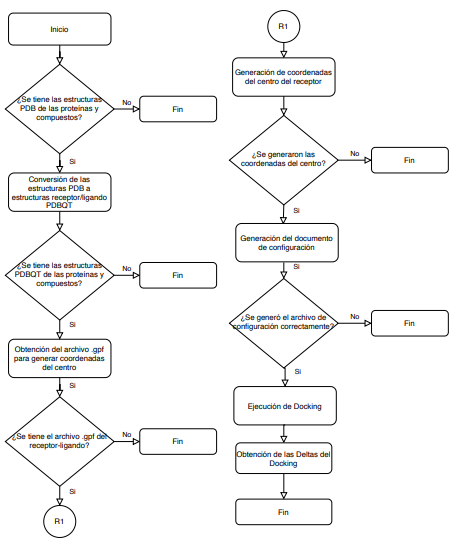
\includegraphics[scale=.65]{Capitulo4/Documentos/imagenes_entorno/docking-flujo.png}
    \caption{Flujo que sigue SysPAF para realizar el proceso de \textit{Docking}.}
    \label{flujo_dock}
\end{figure}

}

\subsubsection{Implementación de algoritmos de \textit{Machine Learning}}{
\noindent El uso de algoritmos de Machine Learning permite la generación de modelos para realizar cálculos más rápidos en términos de predicción de la efectividad de los compuestos de estudio.El uso de algoritmos de \textit{Machine Learning} permite la generación de modelos para realizar cálculos más rápidos. Los modelos se obtienen a partir de una regresión lineal múltiple que toma como variables independientes a los valores de las propiedades físicas y químicas de cada medicamento. La variable dependiente está definida por el valor de delta G obtenido del proceso del \textit{Docking}. Luego de obtener los coeficientes de la regresión lineal, estos son almacenados en un archivo el cual contiene todos los modelos para las distintas clasificaciones de medicamentos (cada clasificación constituye un modelo). Una vez definido el modelo, el proceso del \textit{Docking} y de la regresión lineal puede omitirse en caso de volver a tener que realizar un análisis de información en el cual, luego de revisar el archivo donde se almacenan los modelos, se encuentre el modelo para la clase de compuestos que se están analizando. La figura \ref{Machine} muestra una ilustración del proceso previamente descrito.

\begin{figure}[H]
    \centering
    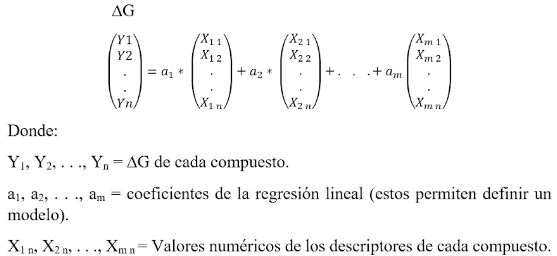
\includegraphics[scale=0.70]{Capitulo4/Documentos/imagenes_entorno/regresion_lineal.png}
    \caption{Forma de implementar la regresión lineal y su relación con los resultados del \textit{Docking}.}
    \label{Machine}
\end{figure}
\noindent Una vez que la regresión lineal es finalizada, el sistema guarda dicho modelo en una carpeta el cual puede recuperar en caso de que se solicite analizar datos correspondientes a una clasificación que corresponda con algún modelo de regresión lineal existente. Al recuperar el modelo correspondiente, se puede simplemente realizar el proceso de predicción directa de la variable Y, dado que en ese modelo se observan ya los coeficientes y las variables independientes X que están determinadas por los descriptores del nuevo conjunto 0 a analizar.
}
\subsubsection{Precisión del modelo de regresión lineal generado}{
\noindent La evaluación de qué tan acertado es el modelo de regresión lineal que se genera luego de aplicar el algoritmo del mismo nombre se basa en la obtener y medir la influencia de los errores en la exactitud del modelo de regresión lineal. Estos errores, si bien se implementan de manera directa gracias a las herramientas de la biblioteca de python sklearn, requieren de su correcta comprensión para poder entender qué tan exacto es el modelo y por qué.\\
\noindent La estadística ha desarrollado medidas resumidas que toman la colección de residuos del modelo (valor actual - valor esperado) y los condensan en un solo valor que representa la capacidad predictiva del modelo implementado. De estas medidas se han considerado 3: Error Medio Absoluto (MAE, por sus siglas en inglés, Mean Absolute Error), Error Cuadrático Medio (MSE, por sus siglas en inglés, Mean Square Error) y Raíz del Error Cuadrático Medio (RMSE, por sus siglas en inglés, Root Mean Square Error).\cite{16}\\

\noindent El error medio absoluto se obtiene mediante la sumatoria de cada valor absoluto del residual (diferencia entre el valor predicho y el valor esperado), y luego dividiendo entre el número de muestras. Este error  se refiere a la media de los valores absolutos de cada error de predicción en todas las instancias del conjunto de datos de prueba.\\
\noindent Para el caso de error medio cuadrado permite determinar qué tan cerca está una línea de regresión de un conjunto de puntos. Lo hace tomando las distancias desde los puntos hasta la línea de regresión (estas distancias son los "errores") y cuadrándolos. La cuadratura es necesaria para eliminar cualquier signo negativo. También le da más peso a las diferencias más grandes (outliers).\\

\noindent Por último, considerando que el error cuadrático medio es la desviación estándar de los residuos y sabiendo que los residuos son una medida de qué tan lejos están los puntos de datos de la línea de regresión, la raíz del error cuadrático medio es una medida de la dispersión de estos residuos. En otras palabras, dice qué tan concentrados están los datos alrededor de la línea de regresión.\\

\begin{figure}[H]
    \centering
    \includegraphics[scale=0.85]{}
    \caption{Representación matemática del error medio absoluto.}
    \label{ecuaciones}
\end{figure}

\begin{figure}[H]
    \centering
    \includegraphics[scale=0.85]{}
    \caption{Representación matemática del error cuadrático medio.}
    \label{ecuaciones}
\end{figure}

\begin{figure}[H]
    \centering
    \includegraphics[scale=0.85]{}
    \caption{Representación matemática de la raíz del error cuadrático medio.}
    \label{ecuaciones}
\end{figure}

\noindent Los errores previamente definidos se utilizan con la observación de que a menor valor, mejor. Es decir, que estos 3 valores resulten en 0 indicaría que el modelo es perfecto. Las pruebas para obtener estos errores se realizaron con los conjuntos de datos indicados que en anexo X. Y en promedio, de X pruebas se obtuvieron los resultados que ilustra la tabla siguiente.



\begin{longtable}{|c|c|c|c|c|c|}
\caption{Resultados de las mediciones de errores realizadas..}\\ 
\hline
\multirow{}{}{\textbf{Clasificación} } & \multicolumn{2}{c|}{\textbf{Número de muestras} } & \multirow{}{}{\textbf{MAE} } & \multirow{}{}{\textbf{MSE} } & \multirow{}{}{\textbf{RMSE} }  \\* 
\cline{2-3}
                                         & \textbf{Entrenamiento} & \textbf{Prueba}          &                                &                                &                                  \endfirsthead 
\hline
Anti-inflamatorio                        & 12                     & 4                        & 0.471                          & 0.472                          & 0.687                            \\ 
\hline
Antiviral                                & 4                      & 2                        & 2.583                          & 6.673                          & 2.583                            \\ 
\hline
Antiandrogénico                          & 2                      & 1                        & 0.82                           & 0.67                           & 0.82                             \\ 
\hline
Cardiovascular                           & 6                      & 2                        & 6.903                          & 72.383                         & 8.507                            \\ 
\hline
Antifúngico                              & 5                      & 2                        & 6.230                          & 39.48                          & 6.272                            \\ 
\hline
Antihipertensivo                         & 18                     & 5                        & 4.934                          & 39.784                         & 6.307                            \\ 
\hline
Antiparasitario                          & 7                      & 2                        & 0.46                           & 0.313                          & 0.56                             \\ 
\hline
Antibiótico                              & 4                      & 2                        & 2.353                          & 10.124                         & 3.181                            \\ 
\hline
Antiepiléptico                           & 5                      & 2                        & 0.03                           & 0.001                          & 0.032                            \\ 
\hline
Anticoagulante                           & 5                      & 2                        & 0.334                          & 0.133                          & 0.364                            \\ 
\hline
\textbf{Total}                           & \textbf{68}            & \textbf{24}              & \textbf{2.511}                 & \textbf{17.003}                & \textbf{2.931}                   \\
\hline
\end{longtable}

\noindent De estos resultados se puede decir que el modelo generado tiene un margen de error de 2.5 unidades, esto es, la variación entre el valor que se espera obtener y el valor que puede predecir el modelo está definida en un rango de 0 a 2.5, y considerando la cantidad de pruebas, se puede concluir que el modelo es eficaz.\\

\noindent Algo muy importante que se debe mencionar es que el modelo de regresión lineal depende en gran medida de la calidad y la cantidad de datos proporcionados. Un modelo con muchas variables independientes para trabajar pero que son pobres en cuanto a la relación cualitativa de estas variables con las variables dependientes resultan en un modelo predictivo poco preciso, por otro lado un modelo donde las variables dependientes tengan mucha influencia en la variable dependiente además de grandes muestras de información para entrenar y probar el modelo derivan en la generación de un modelo más preciso y robusto.
}

%%%%%%%%%%%%%%%%%%%%%%%%%%%%%%%%%%%%%%%%%%%%%%%%%%%%%
\subsection{Generación de resultados}
\subsubsection{Diseño de interfaces}
\noindent La interfaz de despliegue de resultados fue desarrollada con la finalidad de que el usuario pueda visualizar los resultados obtenidos por el sistema, los resultados están desplegados en una tabla de dos columnas, la columna uno lleva por nombre “Compuesto”, donde se en-lista el nombre de cada compuesto, la columna dos tiene el nombre de “Efectividad”, esta muestra los efectos que tuvo el compuesto para “destruir” la proteína, está  representada numéricamente. 

\begin{figure}[H]
    \centering
    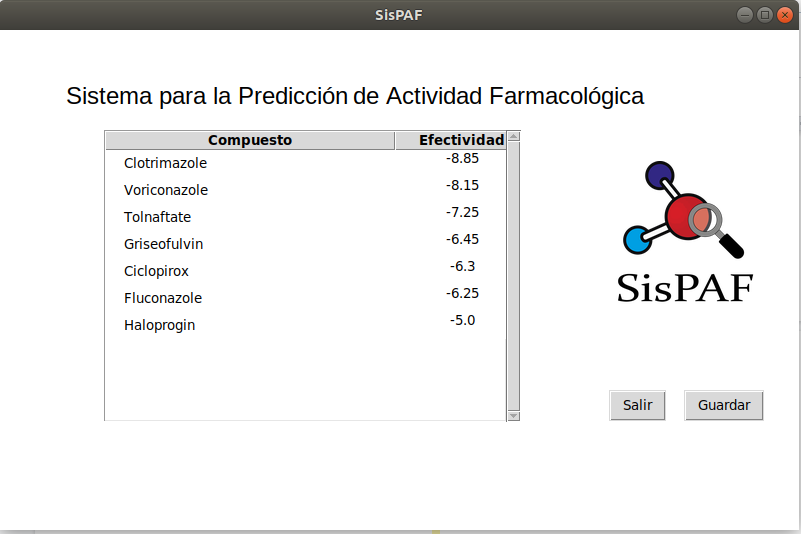
\includegraphics[scale=0.52]{Capitulo4/Documentos/imagenes_generacion/imagen-2-2-7-2.png}
    \caption{Despliegue de resultados.}
    \label{Des_Res}
\end{figure}

\noindent La columna “Efectividad” nos ayudará a ordenar los resultados, ya que se tomará el valor más alto y este será nuestro punto de partida para desplegar nuestros resultados de forma descendente.

\subsubsection{Ordenamiento de resultados:}
\noindent Para el ordenamiento de los resultados, utilizamos una estructura de datos llamada “diccionario” en python, dicha estructura soporta cualquier tipo de dato como enteros, cadenas, listas e incluso otras funciones. La ventaja de utilizar este tipo de estructura es el poder identificar cada elemento por una clave (key) ya que está dada por duplas.

\noindent Donde tomamos el nombre del compuesto como la llave de la dupla y la efectividad como el valor. Para acceder a cada uno de los valores del diccionario de datos, es necesario poner el nombre de la clave (compuesto), lo cual nos permite eliminar la redundancia de datos, ya que esta estructura no guarda datos duplicados.

\subsubsection{Construcción de archivo de resultados:}
\noindent La Para evitar una pérdida de datos, se definió una función que nos permite guardar los resultados obtenidos por el sistema en un archivo txt, dicho archivo se encuentra guardado en una carpeta que lleva por nombre “Resultados” y a su vez este lleva por nombre “Resultados\_Proyecto.txt”. El archivo contiene una estructura similar a la tabla que se muestra en la interfaz de despliegue de resultados y de igual manera está ordenada de mayor a menor efectividad.

\begin{figure}[H]
    \centering
    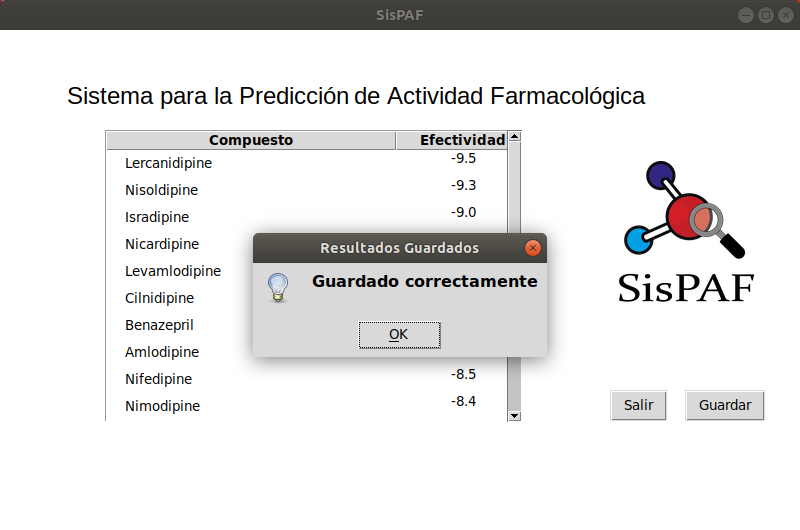
\includegraphics[scale=0.52]{Capitulo4/Documentos/imagenes_generacion/imagen-2-2-8-1.png}
    \caption{Ejemplo de archivo guardado.}
    \label{fig:my_label}
\end{figure}

\subsubsection{Alertas y errores:}
\noindent La interfaz de “despliegue de resultados” cuenta con dos tipos de alertas, las cuales se muestran al efectuar una interacción específica con el sistema, describiremos a continuación dichas alertas de manera individual:

\noindent\textit{Resultados guardados:}\\

\noindent El sistema SisPAF muestra una alerta, cuando el documento fue guardado correctamente, esta acción surge de dar clic en el botón “Guardar” de la interfaz. El objetivo principal de desarrollar esta funcionalidad es notificar al usuario que la acción que realizó fue efectuada con éxito.\\

\begin{figure}[H]
    \centering
    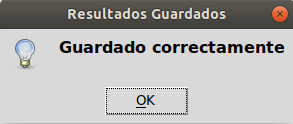
\includegraphics[scale=0.85]{Capitulo4/Documentos/imagenes_generacion/manual_3.png}
    \caption{Resultados guardados correctamente}
    \label{resultados_guard}
\end{figure}

\noindent \textit{Resultados no guardados:}\\

\noindent El sistema SisPAF muestra una alerta que nos permite decidir si seguir con la acción que el usuario seleccionó, dicha acción puede estar descrita por un cierre forzado del sistema, dar clic en el botón “Inicio” o seleccionar el botón de “Salir” que fue implementado en el sistema, todo esto antes de guardar el documento de resultados. El objetivo de esta notificación es poder alertar al usuario de que sus resultados no han sido guardados y de seguir con esta acción podrían perderse y tendrían que ser calculados nuevamente.

\begin{figure}[H]
    \centering
    
\includegraphics[scale=0.85]{Capitulo4/Documentos/imagenes_generacion/manual_4.png}
    \caption{Alerta de acción.}
    \label{resultados_guard}
\end{figure}